\chapter{System Design}

% System Architecture
% UML Diagrams
	% Use Case Diagram
	% Class Diagram
	% Activity Diagram
	% Sequence Diagram

\section{System Architecture}

	\begin{figure}[h]
		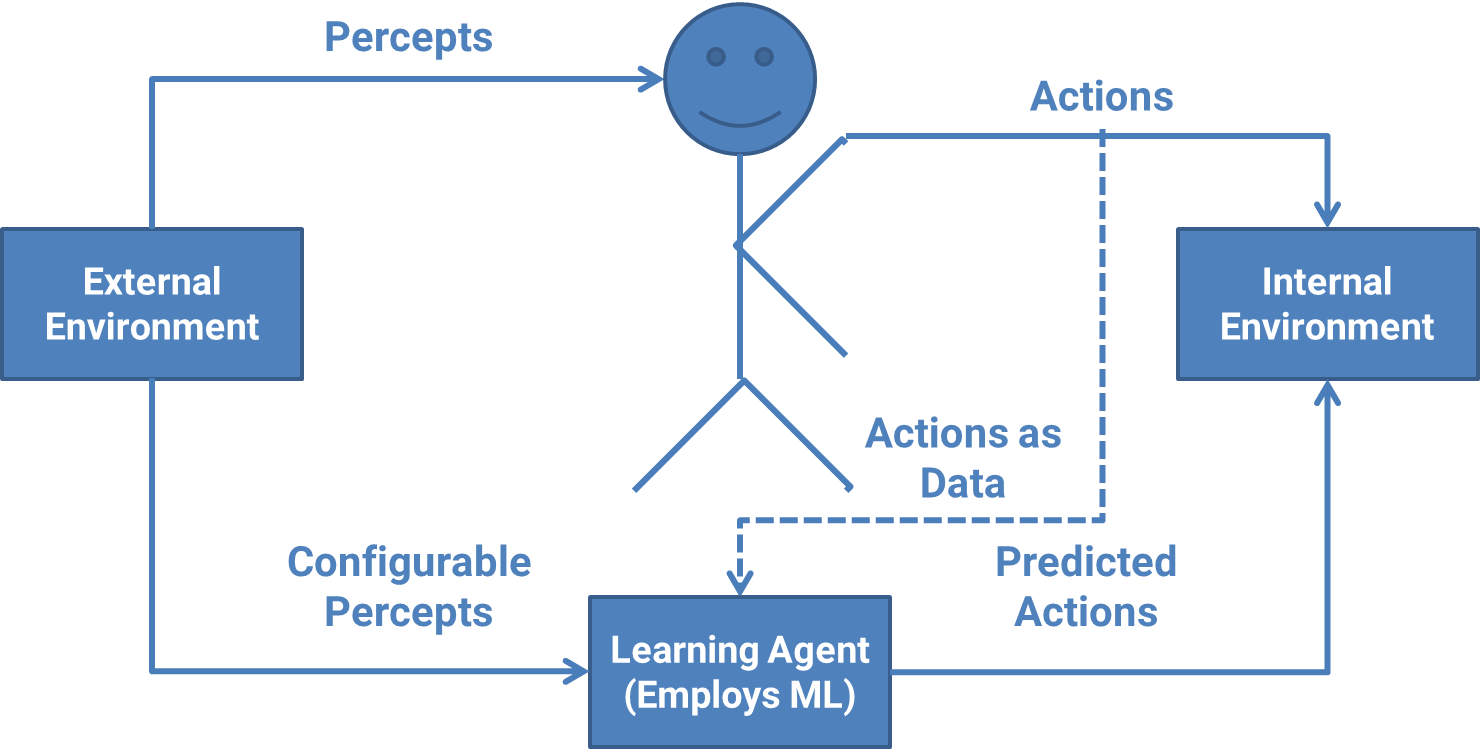
\includegraphics[width=\textwidth]{./Chapter5/system-architecture}
			\caption{System Architecture}
	\end{figure}
	\paragraph{}
	This defines the major elements within our system, their arrangement and interaction. It essentially represents an agent-environment model with the human and the Learning Agent as the two agents.

\section{UML Diagrams}

	\subsection{Use Case Diagram}
	\begin{figure}[H]
	\centering
	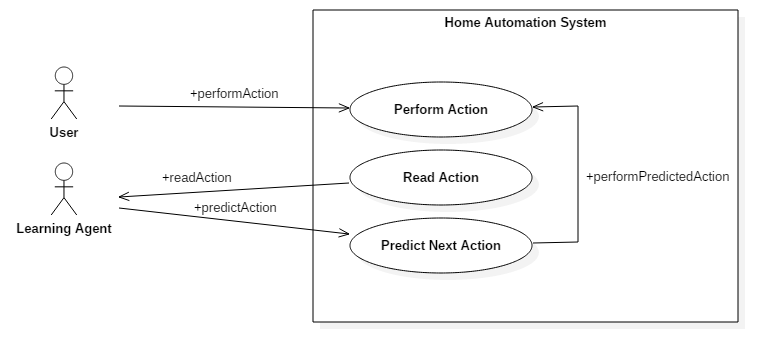
\includegraphics[width=\textwidth]{./Chapter5/UseCaseDiagram}
		\caption{Use Case Diagram}
	\end{figure}
	\paragraph{}
	This represents the various use cases that are possible in our system. The human user is the primary actor which may perform certain actions to initiate learning in a secondary learning agent that mimics the user's usage patterns.
	
	\subsection{Class Diagram}
	\begin{figure}[H]
	\centering
	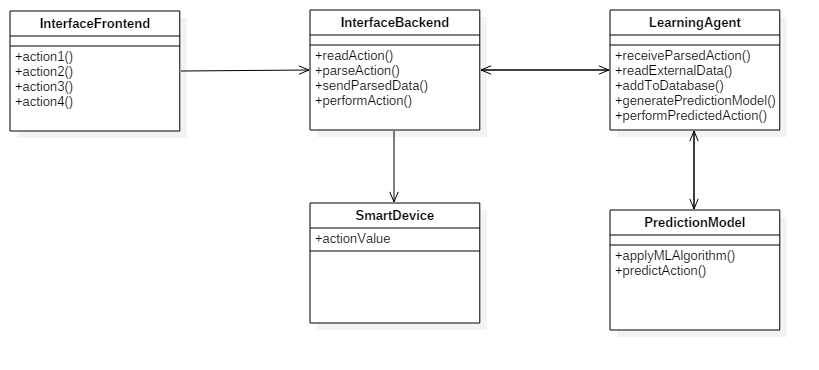
\includegraphics[width=\textwidth]{./Chapter5/ClassDiagram}
		\caption{Class Diagram}
	\end{figure}
	
	\paragraph{}
	This abstracts the major entities within our system as classes and shows the features they offer and the relationship between them.

	\subsection{Activity Diagram}
	\begin{figure}[H]
	\centering
	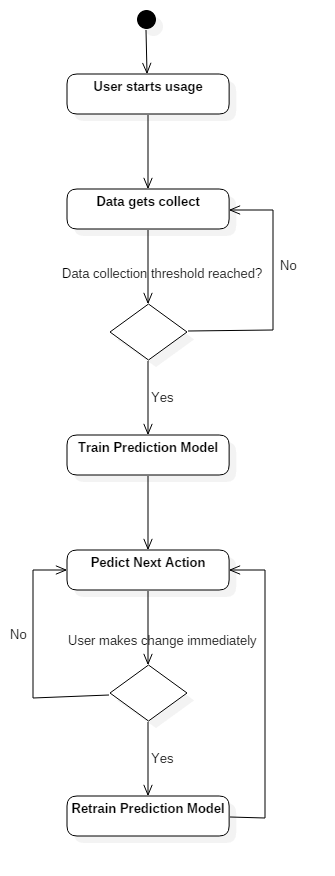
\includegraphics[scale=0.5]{./Chapter5/ActivityDiagram}
		\caption{Activity Diagram}
	\end{figure}
	\paragraph{}
	The activity diagram shows the flow of control through the process of our system. This system is designed to be non-terminating, so there is no halt in the flow. The system improves itself continually by realizing incorrect predictions.
	
	\subsection{Sequence Diagram}
	\begin{figure}[H]
	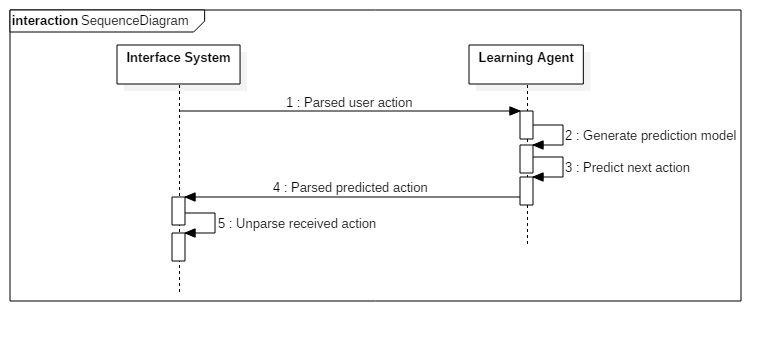
\includegraphics[width=\textwidth]{./Chapter5/SequenceDiagram}
		\caption{Sequence Diagram}
	\end{figure}
	\paragraph{}
	It shows the flow of objective-critical data and signals between some major entities within the system.


\begin{comment}
\begin{figure}
	\includegraphics[width=\textwidth]{Flower}
		\caption{A Flower}
\end{figure}
\end{comment}